% Full-width, self-contained cover graphic, matching the companion paper.
\begin{minipage}{\textwidth}
\centering
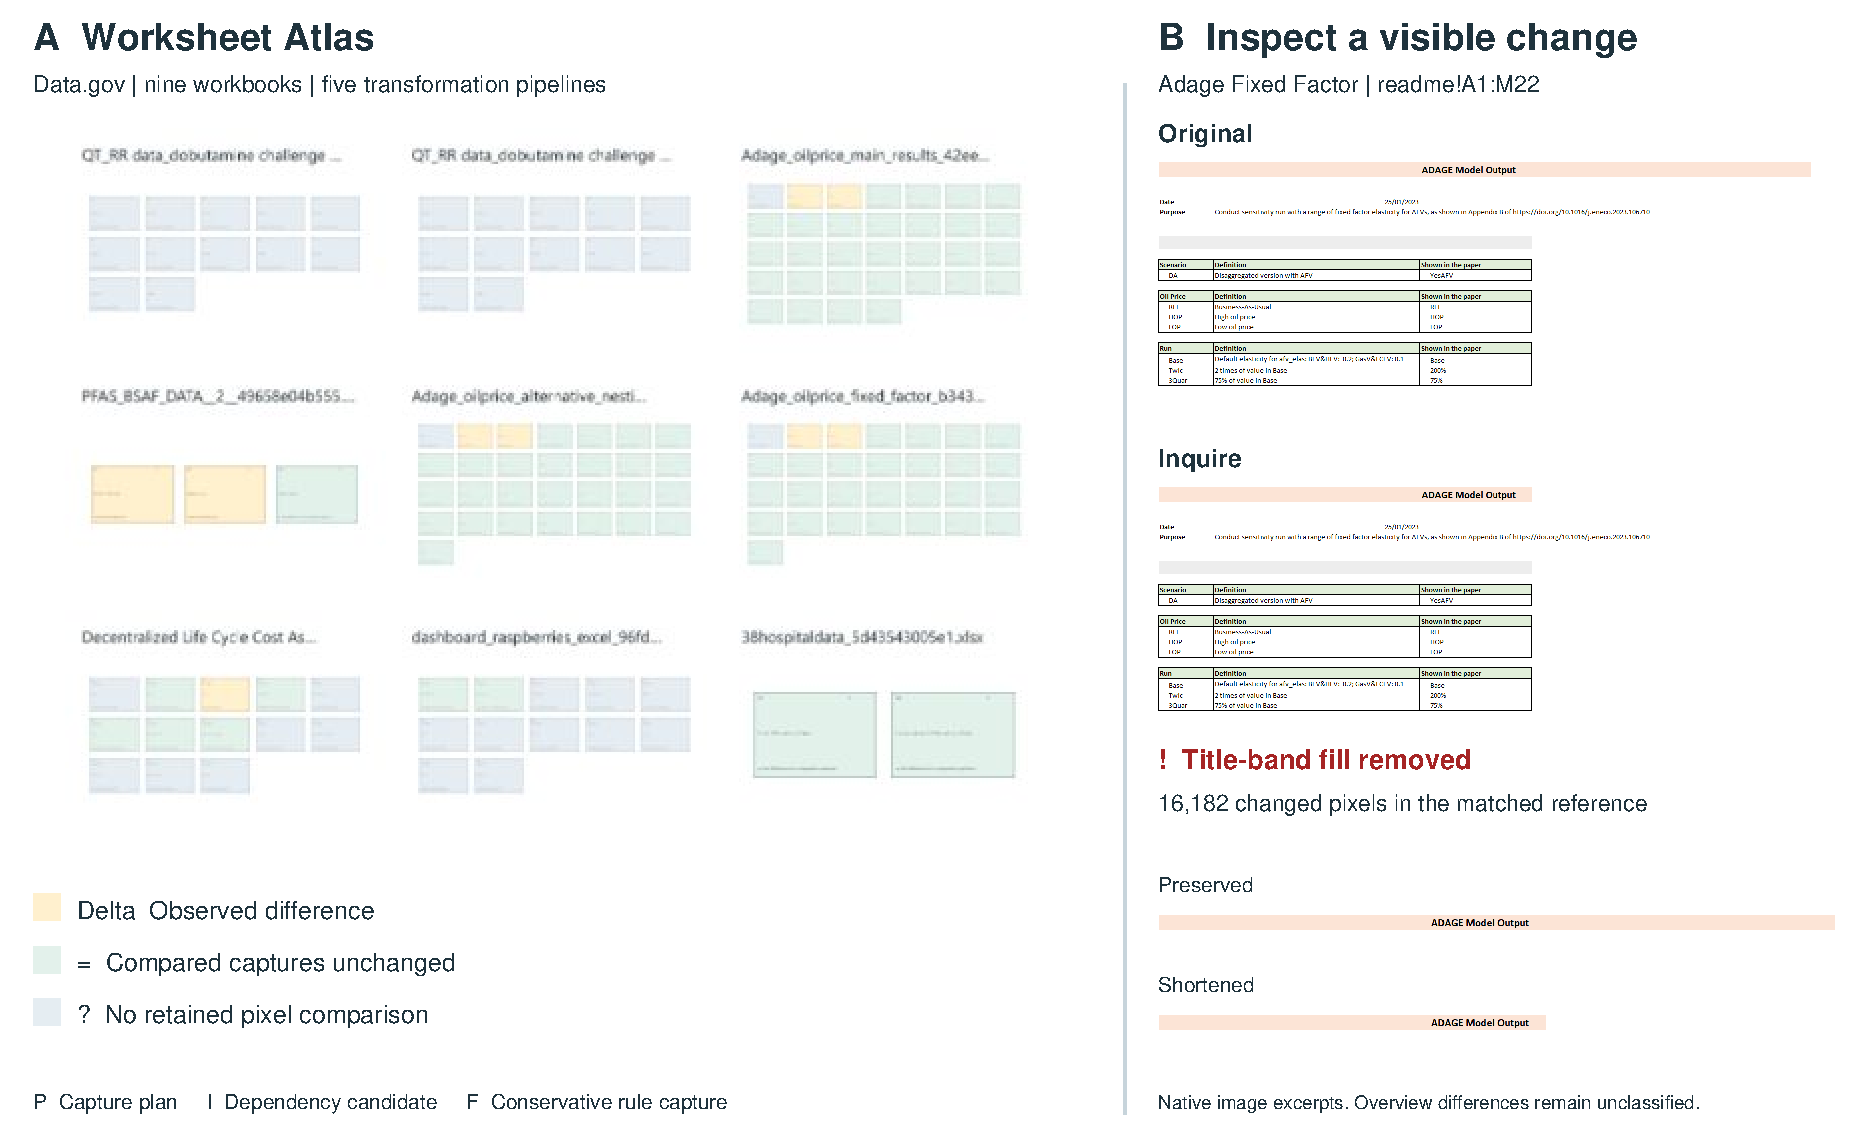
\includegraphics[width=.995\textwidth]{figures/atlas-cover.pdf}
\makeatletter
\def\@captype{figure}
\makeatother
\caption{From worksheet-level evidence to native image inspection. The left
view shows nine Data.gov workbooks and their 144 known sheets. Amber marks
recorded differences with unclassified cause, green denotes unchanged compared
captures, and blue-gray retains missing pixel coverage. Planning badges retain
recorded decisions independently of the outcome. The right view enlarges a
verified Adage title-band change in Inquire. The matched reference has 16,182
changed pixels. The displayed extent also remains shortened in Check Performance
and NXPowerLite, while SheetShrink and XLStylesTool preserve it. These grouped
observations concern this reference range.}
\label{fig:atlas-stage09}
\end{minipage}
\par\medskip
